%%%%%%%%%%%%%%%%%%%%%%%%%%%%%%%%%%%%%%%%%%%%%%%%%%%%%%%%%%%%%%%%%%%%%%%%

%%% LaTeX Template for AAMAS-2021 (based on sample-sigconf.tex)
%%% Prepared by Natasha Alechina and Ulle Endriss (version 2020-08-06)

%%%%%%%%%%%%%%%%%%%%%%%%%%%%%%%%%%%%%%%%%%%%%%%%%%%%%%%%%%%%%%%%%%%%%%%%

%%% Start your document with the \documentclass command.
%%% Use the first variant below for the final paper.
%%% Use the second variant below for submission.

\documentclass[sigconf]{acmart} 

%%% Load required packages here (note that many are included already).

\usepackage{balance} % for balancing columns on the final page
% \usepackage{booktabs} % For formal tables
\usepackage{graphics} % for pdf, bitmapped graphics files
\usepackage{epsfig} % for postscript graphics files
\usepackage{mathptmx} % assumes new font selection scheme installed
\usepackage{times} % assumes new font selection scheme installed
\usepackage{amsmath} % assumes amsmath package installed
\usepackage{amssymb}  % assumes amsmath package installed
% \usepackage{booktabs} % For formal tables
\usepackage{graphicx}
\usepackage{subcaption}
\usepackage{hyperref}

%%%%%%%%%%%%%%%%%%%%%%%%%%%%%%%%%%%%%%%%%%%%%%%%%%%%%%%%%%%%%%%%%%%%%%%%


% Copyright
%\setcopyright{none}
%\setcopyright{acmcopyright}
\setcopyright{acmlicensed}
%\setcopyright{rightsretained}
%\setcopyright{usgov}
%\setcopyright{usgovmixed}
%\setcopyright{cagov}
%\setcopyright{cagovmixed}


% DOI
\acmDOI{10.1145/nnnnnnn.nnnnnnn}

% ISBN
\acmISBN{978-x-xxxx-xxxx-x/YY/MM}

% Conference
\acmConference[GECCO '21]{the Genetic and Evolutionary Computation Conference 2021}{July 10--14, 2021}{Lille, France}
\acmYear{2021}
\copyrightyear{2021}

%\acmArticle{4}
\acmPrice{15.00}

%%%%%%%%%%%%%%%%%%%%%%%%%%%%%%%%%%%%%%%%%%%%%%%%%%%%%%%%%%%%%%%%%%%%%%%%

%%% Use this command to specify the title of your paper.

\title[Spatial Defence for CDM]{A  Bio-Inspired  Spatial  Defence  Strategy  for  Collective  Decision  Making in Self-Organized  Swarms}

%%% Provide names, affiliations, and email addresses for all authors.

\author{Judhi Prasetyo}
\affiliation{
  \institution{Universit\'e de Namur and  Middlesex University Dubai}}
\email{judhiprasetyo@unamur.be}

\author{Giulia De Masi}
\affiliation{
  \institution{Technology Innovation Institute and Khalifa University}
  \city{Abu Dhabi, UAE}}
\email{giulia.demasi@tii.ae}

\author{Raina Zakir}
\affiliation{
  \institution{Middlesex University Dubai}
  \city{Dubai, UAE}}
\email{rz114@live.mdx.ac.uk}

\author{Muhanad Alkilabi}
\affiliation{
  \institution{Universit\'e de Namur}
  \city{Namur, Belgium}}
\email{mhmmoham@unamur.be}


\author{Elio Tuci}
\affiliation{
  \institution{Universit\'e de Namur}
  \city{Namur, Belgium}}
\email{elio.tuci@unamur.be}

\author{Eliseo Ferrante}
\affiliation{
  \institution{Technology Innovation Institute and Vrije Universiteit Amsterdam}
  \city{Abu Dhabi, UAE}}
\email{e.ferrante@vu.nl}

%%% Use this environment to specify a short abstract for your paper.

\begin{abstract}
Collective decision-making is a process where individuals in a swarm have to reach consensus on a decision using only local interactions without any centralized or external control. In the context of the best-of-$n$ problem - whereby the consensus on the best option among a set of $n$ alternative is sought - it has been shown that consensus to one option (e.g. the best one) can be reached if individuals disseminate that option more than the others.
Besides being used as a mechanism to modulate positive feedback to achieve good collective decision, long dissemination times could potentially also been used in an adversarial way, whereby adversarial swarms could infiltrate the system and propagate bad decisions using aggressive dissemination strategies. Motivated by the above scenario, in this paper we propose a bio-inspired defence strategy that allows the swarm to be resilient against options that can be disseminated for longer times. This strategy mainly consists in reducing the mobility of the agents that are associated to options that can be disseminated for a shorter amount of time, allowing the swarm to converge to this option. 
We study the effectiveness of this strategy using two classical decision mechanisms, the voter model and the majority rule, showing that the majority rule is, at least in the current setting, necessary for this strategy to work. The strategy has also been validated on a real Kilobots proof of concept experiment. 

\end{abstract}

%%% The code below was generated by the tool at http://dl.acm.org/ccs.cfm.
%%% Please replace this example with code appropriate for your own paper.


%%% Use this command to specify a few keywords describing your work.
%%% Keywords should be separated by commas.

\keywords{Collective decision-making, Best-of-n problem, spatial defence}

%%%%%%%%%%%%%%%%%%%%%%%%%%%%%%%%%%%%%%%%%%%%%%%%%%%%%%%%%%%%%%%%%%%%%%%%

%%% Include any author-defined commands here.
         
\newcommand{\BibTeX}{\rm B\kern-.05em{\sc i\kern-.025em b}\kern-.08em\TeX}

%%%%%%%%%%%%%%%%%%%%%%%%%%%%%%%%%%%%%%%%%%%%%%%%%%%%%%%%%%%%%%%%%%%%%%%%

\begin{document}

%%% The following commands remove the headers in your paper. For final 
%%% papers, these will be inserted during the pagination process.

\pagestyle{fancy}
\fancyhead{}

%%% The next command prints the information defined in the preamble.

\maketitle 

%%%%%%%%%%%%%%%%%%%%%%%%%%%%%%%%%%%%%%%%%%%%%%%%%%%%%%%%%%%%%%%%%%%%%%%%

\section{Introduction}

\begin{figure*}[t]
  \centering
  \subfloat[]{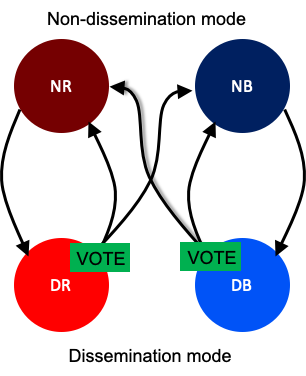
\includegraphics[width=0.3\textwidth]{images/StateMachine.png}
  \label{fig:statemachine}}
  \hfill
  \subfloat[]{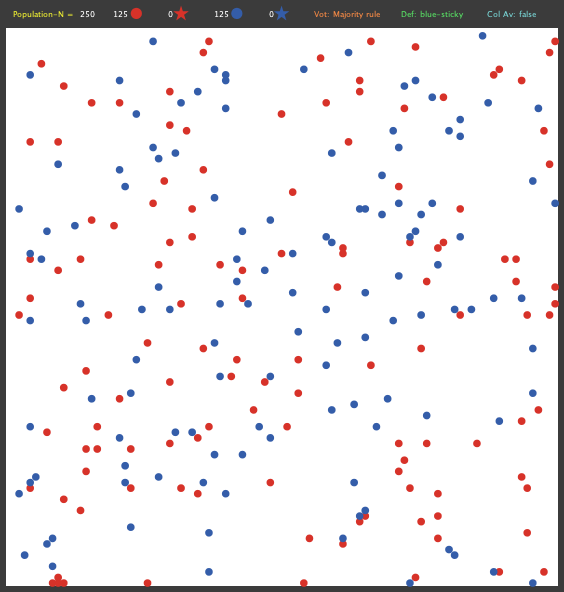
\includegraphics[width=0.4\textwidth]{images/arena.png}
  \label{fig:arena}}
  \hfill
  \caption{Panel $a$: Probabilistic finite state machine. $NR$, $NB$ , $DR$  and $DB$ represent the non-dissemination and dissemination states, for RED and BLUE agents respectively.  Panel $b$: Screenshot of the simulation arena. %This image is taken from NetLogo software
  }
  \label{fig:arena_and_method}
\end{figure*}
In the last years, swarm robotics is getting momentum, thanks to the availability of cheaper and smaller agents, with available integrated sensors and communication devices\cite{book:Hamann:2018}.  While  swarms of robots that are either manually controlled or operated semi-autonomously using external sensing and/or computation are nowadays well established, the realization of fully autonomous swarms of robots, with sensing and computation realized fully on-board, is still under investigation. The field of swarm robotics defines a swarm as a potentially large group of robots that operate without any centralized or external control, but by only relying on local interaction and communication~\cite{brambilla|ferrante|birattari|dorigo:2013}. Swarms of robots are potentially very beneficial mostly  in GPS denied environment, where the external control is prevented by the unavailability of communications or GPS. 

One of the basic capability sought in a robot swarm is attainment of collective decisions~\cite{book:Bonabeau1999SwarmI,Valentini2017Review}. Many other collective behaviours can be seen as an instance of collective decision making, such as deciding a common direction of motion~\cite{FerranteNOALIGN}, or a common location in the environment to explore at~\cite{correll|martinoli:2011}. A special case of collective decision making is represented by the best-of-$n$ problem, whereby there is a discrete number $n$ of options and the swarm has to achieve consensus on the best of them. A  perspective on the best-of-$n$ problem can be found in~\cite{Valentini2017Review}, whereby it is argued that two factors are key in collective decision-making: the intrinsic qualities associated to the different options~\cite{FontLlenas:ANTS:2018,valentini|hamann|dorigo:2014,valentini|ferrante|hamann|dorigo:2015}, or the cost associated to each option in case of asymmetrical environments~\cite{montesdeoca|ferrante|scheidler|pinciroli|birattari|dorigo:2011,scheidler|brutschy|ferrante|dorigo:2015,BruSchFer-etal2012:iros}. In this view, the \emph{best} option the swarm has to choose can be the one associated to the highest quality, to the lowest cost, or a compromise between these two. In general, across all those cases, the key factor determining to what option the swarm will converge is positive feedback: if robots observe, on average, more frequently one option, the swarm will more likely converge to this option. This happens because the initial symmetry (equal distribution of options) will more likely break in favour of the most frequently observed option, and subsequently this option will be even more abundant (positive feedback), thus biasing even further the consensus, and so on. This "frequency of exposure", or modulation of positive feedback, for one option can be environment-dependent and uncontrolled (passive modulation of positive feedback) in case of asymmetric environmental cost (e.g. in tasks in which the physical path to each option differs~\cite{montesdeoca|ferrante|scheidler|pinciroli|birattari|dorigo:2011}), or can be instead controlled by modulating the frequency of dissemination (active modulation of positive feedback, e.g. via communication) as a control parameter, for example by having it proportional to the quality of the option assuming it can be measured~\cite{valentini|ferrante|hamann|dorigo:2015}. While in general the best-of-$n$ collective decision making is not adapting to sudden changes of the environments, it has been demonstrated that such adaptability can be achieved by introducing a  limited number of stubborn individuals~\cite{prasetyo2018, DeMasiHTC2020}. 

Importantly, the  mechanism for active modulation of positive feedback opens the possibility for it to be used not only as mechanism to achieve the best option, but also as a way to perform  attacks by adversarial swarms wishing to manipulate the information or the mission of the focal swarm. This motivates the need to perform studies aiming at finding defence strategies whereby swarms can converge to an option even if this is less frequently disseminated compared to the one advertised by the attacker. This problem is analogous to the one encountered in other social systems, such as social media where automated bots are able to manipulate people's opinion by a massive media campaign observable by many gullible individuals\cite{Ferrara2017MeasuringSS}. On the application perspective, guaranteeing the safety of operations of swarms of robots outside the lab is emerging as a crucial issue \cite{Hunt2020, Reina2020, Jones2020}.
% answer to Review 1-1 below
Several approaches of defence strategy are understudy, from applications of blockchain technology \cite{Strobel2020_blockchain} to complex network analysis to evaluate the resiliency of the swarm \cite{Liu2020}.

% The objective of this experiment is to study various defensive strategies of robots in a group of swarm to defend its opinion against attacks from other robots with different opinions in a battle of decision making. 

% Agents who have the inferior quality option must be able to defend their opinion against the influence of agents promoting the superior quality option. 

In this paper, we propose a defence mechanism inspired by the one used by
stingless bees %of resin plastering or “sticking” intruders
\cite{Nieh2005,Gastauer2011} and we demonstrate it in a multi-agent model as well as on a real kilobot proof of concept. The defence strategy 
is based on a reduction of the mobility pattern: the "defending" agents  are allowed to simply remain at the current position, while attackers are continuously moving attempting to spread their opinion within the swarm. This strategy is capable of inverting the expected final consensus, allowing the agents with lower dissemination capability to win and drive the consensus.  Two voting mechanisms, used by the agents to change opinion based on neighbors opinion, are considered: the voter model and the majority rule. The problem of designing defence mechanisms for self-organized robot swarms is relatively new, one recent example is the work in~\cite{PrimieroEtAl:2018} where a similar, non-spatial, defence mechanism was designed for the case where dissemination time was symmetric. 

Our study is performed using simplified multi-agent simulations and validated on an experiment involving real robots (in this case, Kilobot robots \cite{Rubenstein2012kilobot}).

The remaining of the paper is organized as follows. In Section~\ref{sec:method}, we define more formally the problem and the methodology used to model it; in Section~\ref{sec:expsetup}, we present the experimental setup of both simulations and real robot experiment; in Section~\ref{sec:results}, we discuss the results and the validation with the real robots; in Section~\ref{sec:conclusions} we discuss the findings in the light of a larger picture.

% In this paper, we analyze the effect of  spatial correlation as a result of non-uniform aggregation affects consensus in swarm of agents with various population sizes. Inspired by the strategy used by
% stingless bees 
% \cite{Nieh2005,Gastauer2011} to defend their nest. When attacked, stingless bees will stay in their position and throw sticky resin to the enemy, render them immobile. This strategy can be seen as non-uniform aggregation that introduce spatial correlation. We apply similar strategy on a swarm of autonomous agents in the context of Best-of-$n$ problem scenario where a group of agents need to defend their opinion against the influence of other group. The strategy adaptation is based on modification of the mobility pattern: the "defending" robots  are allowed to simply remain at the current position, while "attackers" are continuously moving attempting to spread their opinion within the swarm. This strategy is capable of inverting the expected final consensus, allowing the robots with lower dissemination capability to win and drive the consensus.  Two voting mechanisms, used by the robots to change opinion based on neighbors opinion, are considered: the voter model and the majority rule. 

% %--- reference to Seeley's experiment below
% Although many robot swarms experiments has been conducted, especially those related to Collective decision-making modeled after the work of~\cite{seeley:2010}, the problem of designing defence mechanisms for self-organized robot swarms is relatively new. One recent example is the work in~\cite{PrimieroEtAl:2018} where a similar  defence mechanism was designed for the case where dissemination time was symmetric. However, this design is non-spatial.
% % Addressing important properties of symmetry breaking in the CDM process using stochastic approach.
% % Hamann, H. et al. (2010) ‘A Model of Symmetry Breaking in Collective Decision-Making. Focus on symmetry breaking but not on defense strategy.
% A work in~\cite{hamann:2010} addressed important properties of symmetry breaking in the CDM process using stochastic approach, while our research is focused on analysing various defence mechanisms that can be used in symmetry breaking.
% % -------
% % Multi Robots cooperation mechanism inspired by biological immune systems
% % Razali, S. (2014) ‘Immune Systems Inspired Multi-Robot. This is also a bio inspired research on defense mechanism but the focus is to improve communication reliability of  multi-robot systems that can be compromised due to complexity and dynamic environment.
% Another bio inspired research on defence mechanism by  \cite{Razali2014} is related to multi-robot systems with the goal of improving communication reliability that can be compromised due to complexity and dynamic environment; while our research context is in reaching consensus.
% %----------

% Our study is performed using simplified multi-agent simulations and validated on an experiment involving real robots (in this case, kilobot robots).

% The remaining of the paper is organized as follows. In Section~\ref{sec:method}, we define more formally the problem and the methodology used to model it; in Section~\ref{sec:expsetup}, we present the experimental setup of both simulations and real robot experiment; in Section~\ref{sec:results}, we discuss the results and the validation with the real robots; in Section~\ref{sec:conclusions} we discuss the findings in the light of a larger picture.


%\textbf{Here}

% Modeled as agents that stick in their original position (immobile) throughout the experiment and influence the opposing agent to switch side (and stick on their position). 

% There are two options to choose: Red and Blue. Red robots are the attackers. Blue robots want to keep their opinion and drive the consensus to their opinion.  

% Our scenario can be represented as a best-of-$n$ problem, where a swarm of agents is designed to be able to choose the bet among a set of $n$ options, which have -using a vocabulary familiar in collective decision making models- different qualities. Since the time of dissemination is proportional to the quality, the quality of RED (BLUE) option  in the present case can be interpreted as the tendency of RED (BLUE) to be aggressive. Therefore, contrarily to what is usually done in the studies of best-of-$n$, in the current paper we want to identify a strategy (if any) to make the swarm reach a consensus to the option with lower quality. In other words, we want to know if this defensive strategy can help the Blue option to win against the Red option. 


   

% \section{RELATED WORKS}
% Literature review goes here.

% Addressing important properties of symmetry breaking in the CDM process using stochastic approach.
% Hamann, H. et al. (2010) ‘A Model of Symmetry Breaking in Collective Decision-Making. Focus on symmetry breaking but not on defence strategy.

% Multi Robots cooperation mechanism inspired by biological immune systems
% Razali, S. (2014) ‘Immune Systems Inspired Multi-Robot. This is also a bio inspired research on defence mechanism but the focus is to improve communication reliability of  multi-robot systems that can be compromised due to complexity and dynamic environment.

% Influencing swarm by controlling hubs in a complex network.
% Masuda, N. (2015) ‘Opinion control in complex networks’. This paper addressed similar situation where the researchers try control the outcome of a collective decision-making, but it is done in a complex network environment and using zealot agents. On the other hand, in our experiment the agents are interacting in two dimensional space and there is no zealot agent.


% Primiero, G. et al. (2018) ‘Swarm attack: A self-organized model to recover from malicious communication manipulation in a swarm of simple simulated agents’. This research shows the use of adaptive and non-adaptive probabilistic to minimize effect of attack. While this paper has a close relevance with our research, but it is focused on recovery against attack targeted at swarm communication system rather than strategy to reaching consensus on a collective decision-making.

\begin{table*}[t]
\caption{Experiment Parameters}
\label{params-table}
\centering
\begin{tabular}{|c|c|c|}
\hline
Notation
&
Values
&
Description
\\
\hline
$N$
&
$[100, 250, 500, 750, 1000]$.
&
Swarm Population, total number of robots.\\
\hline
$\rho_{RED}$
&
$[1.0, 1.25, 2.5, 3.75, 5.0, 6.25, 7.5, 8.75, 10]$
&
RED Dissemination Factor.\\
\hline
$\rho_{BLUE}$
&
$[1.0]$
&
BLUE Dissemination Factor.\\

\hline
-
&
["Voter Model","Majority Rule"]
&
Voting methods.
\\
\hline
$k$
&
$[3,5,7]$
&
Minimum number of agents that participate in the voting when using Majority Rule.
\\
\hline
\end{tabular}
\end{table*}


\section{PROBLEM DEFINITION AND METHOD}
\label{sec:method}

We consider a collective decision making-process in a swarm of $N$ agents modeled as the discrete best-of-$n$~\cite{Valentini2017Review}. We consider the case $n=2$, and we label the two options as RED and BLUE. The two options are associated to different dissemination times: the RED option is the \emph{attacker} option and has a longer dissemination time than the BLUE option, the \emph{defender} option.

The dissemination times above are exponentially distributed and each (BLUE or RED) proportional to a parameter that we call \emph{dissemination factor}.  Only the ratio between the two dissemination factors play a role. %, rather then their absolute values [CITARE]. 
To keep the observation simple, the dissemination factor of BLUE has been fixed to the value $1$. Only the RED dissemination factor $\rho_{RED}$ is varied, using values greater or equal to $1$. 
Half of the population is initialized with RED opinion and the other half with BLUE opinion. 
% answer to Review  1-2 below
Agents with RED opinion have dissemination time  proportional to RED option value, and those with BLUE opinion will disseminate proportional to BLUE option value.  
The agents' location are initially randomly distributed.

The agents with the RED opinion implement a random walk and always move freely in an arena with closed bounds and no periodic boundaries. When they do not implement any strategy (here referred to as \emph{No Strategy}), the BLUE agents perform random walk exactly like the agents with the RED option. But, when they implement our novel defence strategy (referred to as \emph{Blue-sticky}), they remain in their initial position. If a RED robot changes opinion after the decision making mechanism, it becomes BLUE  and stops in its last position.  Within the simulations, collision checks are not implemented and individuals may freely collide or overlap with each other, an assumption that does not hold in the real robot experiments.

The robot behavior can be modeled as a Finite State Machine in Fig. \ref{fig:statemachine}. All agents start in a non-dissemination state (NR or NB, for RED and BLUE respectively) and they remain in this state for an  amount of time that is randomly sampled from an exponential distribution with parameter $\tau_{ND} = q = 10$, common to RED and BLUE agents.
Then they transition to a dissemination state (DR or DB), in which they promote their opinion for an amount of time sampled from an exponential distribution with parameter proportional to the dissemination factor $\tau_D= q \cdot \rho_i$, where $q=10$  and  $i \in \{ RED, BLUE \}$, after which they perform \emph{voting} before transitioning again to non-dissemination mode and the cycle repeats. %The rate of the dissemination time for the RED (resp. BLUE) option is equal to \textbf{write}. 
Since, as explained above, we only consider $\rho_{RED} > \rho_{BLUE} = 1$, the dissemination time for the RED option is on average larger than the dissemination time of the BLUE option. In absence of defence mechanisms, this is shown to lead to a positive feedback modulation mechanism that makes the system converge to the RED option with higher probability compared to the BLUE option~\cite{valentini|ferrante|hamann|dorigo:2015}. 

During voting, each robot observes the opinion of nearby disseminating agents and uses this information to determine its next opinion. We consider two voting mechanisms: the voter model and the majority rule. In the voter  model,  agents change their opinion copying the opinion of a random neighbor, while in the majority model  instead agents adopt the opinion of the local majority ($k$ random neighboring agents including the focal robot). Agents who  are in non-dissemination mode will not be visible, hence their opinion will not be counted during the voting. This state (sometimes referred to as \emph{latent} state~\cite{montesdeoca|ferrante|scheidler|pinciroli|birattari|dorigo:2011})  models for example the situation where agents relocate elsewhere in space to assess the quality of the options, or pause the activity of the communication device to save battery.

The simulation runs for a maximum  amount of time $T=1000000$ time steps or terminates early if a stationary consensus state is reached. In this study consensus is always achieved to one of the two options, hence the time limit $T$ was in practice never reached in our experiments. Various values of population size $N$ and dissemination factor ratio $q=\frac{\rho_{RED}}{\rho_{BLUE}} =\rho_{RED}$ are simulated, as reported in Table \ref{params-table}. 
For each set of parameters, the simulation  is repeated $100$ times, and we focus our attention to the percentage of the times the consensus to BLUE is achieved.

\begin{figure*}[t]
  \centering
  \subfloat[]{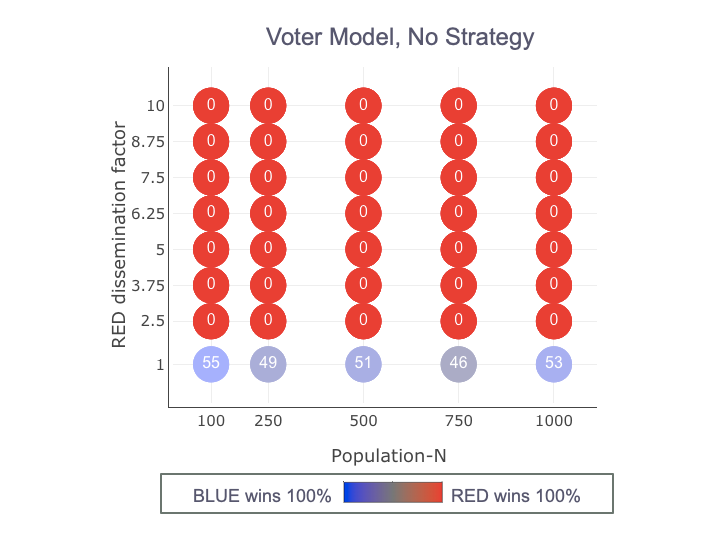
\includegraphics[width=0.49\textwidth]{images/Chart-Voter-NoStrategy.png}
  \label{fig:nostra-voter}}
  \hfill
  \subfloat[]{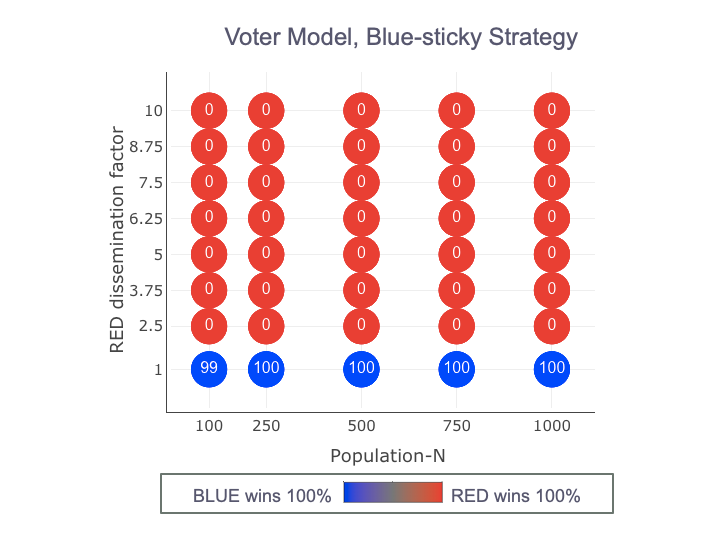
\includegraphics[width=0.49\textwidth]{images/Chart-Voter-BlueSticky.png}
  \label{fig:sticky-voter}}
  \caption{Results with the voter model: (a)  No strategy and (b) Blue-sticky strategy. In both cases, the color code is related to the percentage of consensus: full red represents 100\% of cases of consensus to RED option, full blue represents 100\% of runs where consensus is for BLUE, grey color represents mid-point where BLUE and RED option converge for roughly equal number of runs. The percentage number of BLUE wins (runs) is reported with white characters inside each circle.% symmetrical quality value. %, there is no way for both sides to always win; the consensus always land slightly above or below 50\%. However, when Red quality is higher, Red always win. 
  %(b) \textbf{wrong} With no strategy and symmetrical quality value, there is no way for both sides to always win; the consensus always land slightly above or below 50\%. However, when Red quality is higher, Red always win.
  }
  \label{fig:voter}
\end{figure*}

\begin{figure*}
  \centering
  \subfloat[]{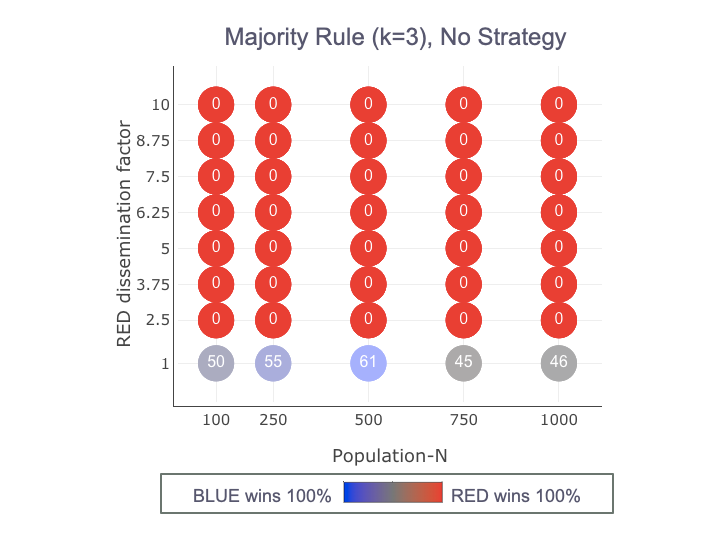
\includegraphics[width=0.49\textwidth]{images/Chart-Maj-k3-NoStrategy.png}
  \label{fig:nostra-k3}}
  \hfill
  \subfloat[]{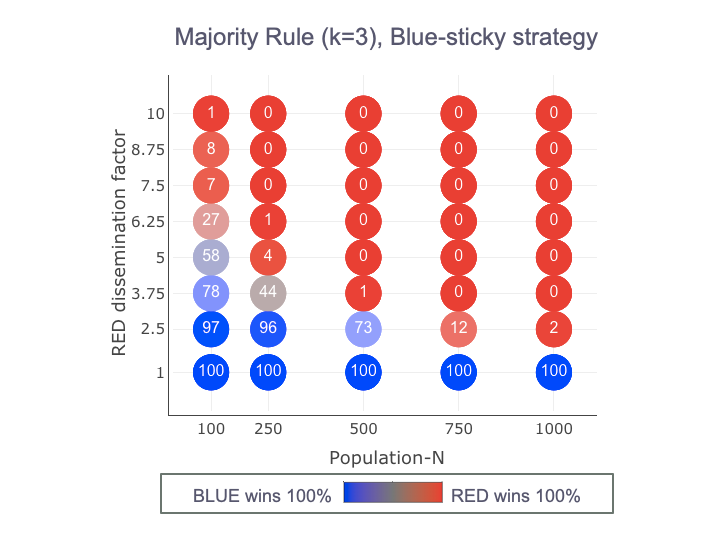
\includegraphics[width=0.49\textwidth]{images/Chart-Maj-k3-BlueSticky.png}
  \label{fig:sticky-k3}}
  \caption{Results with the majority model: (a)  absence of defender strategy  ($k=3$) and (b) defender strategy ($k=3$). This figure uses the same color-code convention used in Figure~\ref{fig:voter}.}
  \label{fig:majority1}
\end{figure*}

%(a) No-strategy, Majority rule (k=3). Similar to Voter model without strategy, in Majority Rule with symmetric quality we get no side that always win. We also did experiments using Majority rule with k=5 and k=7 without strategy and the results are similar to this chart. (b) Blue-sticky defence strategy, Majority rule (k=3). Here the result is getting more interesting as Blue  was able to defeat Red who has up to 2.5 times of the quality (with Population-N = 100 and 200), and managed to prevent Red from winning despite Red quality is 5 times of Blue (with Population-N = 100). As the population grows, Blue's ability to win against Red is decreasing.}
  

\section{EXPERIMENTAL SETUP}
\label{sec:expsetup}
In this section we explain the two setups used for the simulations and for the real robot validation.

\subsection{Simulations}

%   \begin{figure}[thpb]
%       \centering
%       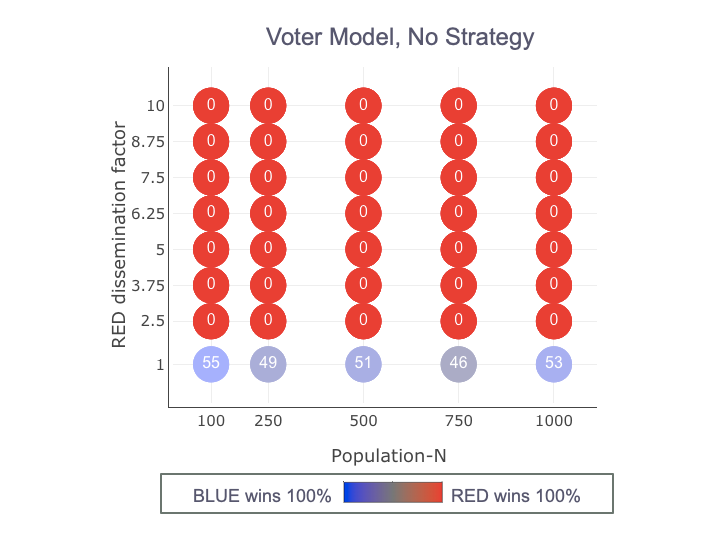
\includegraphics[trim={3cm 0 0 0},clip,scale=0.4]{images/Chart-Voter-NoStrategy.png}
%       \caption{No-strategy, Voter model. With no strategy and symmetrical quality value, there is no way for both sides to always win; the consensus always land slightly above or below 50\%. However, when Red quality is higher, Red always win. }
%       \label{nostra-voter}
%   \end{figure}



%   \begin{figure}[thpb]
%       \centering
%       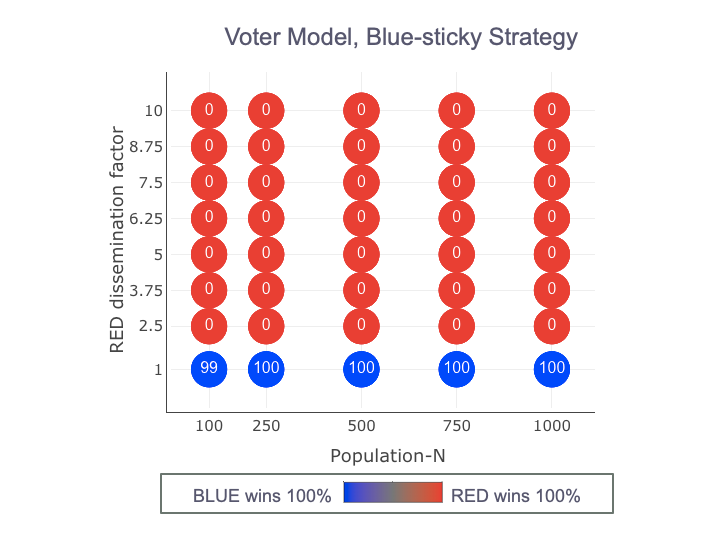
\includegraphics[trim={3cm 0 0 0},clip,scale=0.4]{images/Chart-Voter-BlueSticky.png}
%       \caption{Blue-sticky defence strategy, Voter model. By deploying Sticky defence strategy on Blue option, it is clear that Blue always wins even when the quality value is symmetrical. However with higher Red quality ratio, still there is no chance for Blue to win.}
%       \label{sticky-voter}
%   \end{figure}
 


\begin{figure*}
  \subfloat[]{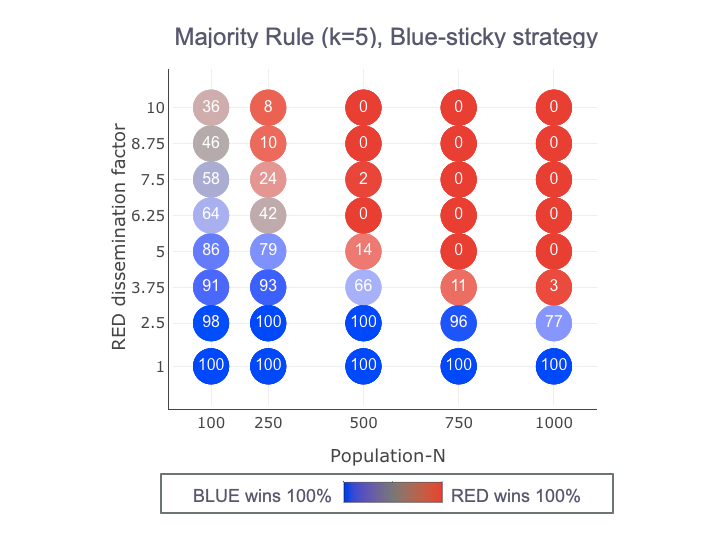
\includegraphics[width=0.49\textwidth]{images/Chart-Maj-k5-BlueSticky.png}
  \label{fig:sticky-k5}}
  \hfill
  \subfloat[]{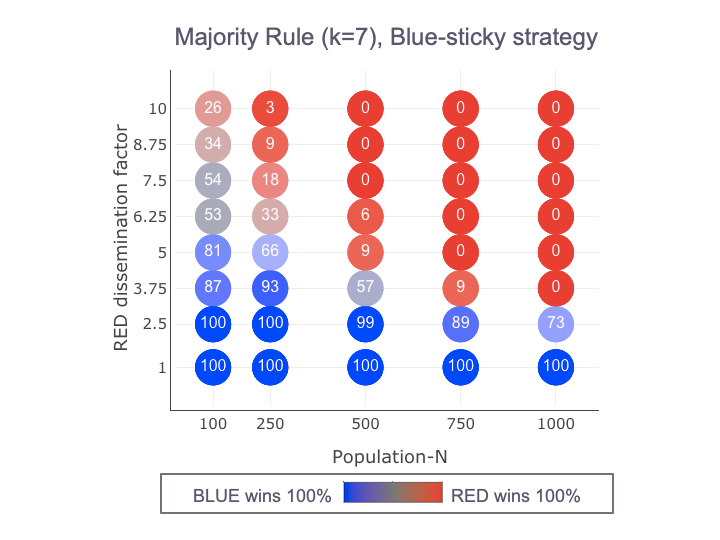
\includegraphics[width=0.49\textwidth]{images/Chart-Maj-k7-BlueSticky.png}
  \label{fig:sticky-k7}}
  \caption{Results with the majority model: (a)  $k=5$ and (b) $k=7$. This figure uses the same color-code convention used in Figure~\ref{fig:voter}.}
  \label{fig:majority2}
\end{figure*}

%(a) Blue-sticky defence strategy, Majority rule (k=5). The ability of Blue to win over Red extends to larger quality ratio as now we see in Population-N = 100 Blue always win at quality ratio of 5 and sometimes win at quality ratio of 7.5, while on Population N=1000 Blue always win at quality ratio of 2.5 as compared to always lose in previous chart with k=3. (b) Blue-sticky defence strategy, Majority rule (k=7). The chart shows more convincing result where Blue managed to win against Red who has the quality ratio 10 times higher with Population-N = 100, while with Population-N=1000, although Red still wins at quality ratio of 5, the shade of the red circle is paler as compared to previously shown in k=3 chart.}
  
The simulations are performed using the Netlogo simulation tool\footnote{\url{https://ccl.northwestern.edu/netlogo/}}. 
Individuals sized 1 square-unit each are placed randomly with no overlap in a 2D simulation arena of 100x100 square units as shown in Fig. \ref{fig:arena}. The swarm sizes considered were $N \in [100, 250, 500, 750, 1000]$. 
RED and BLUE opinion are initially assigned in equal proportion to the $N$ agents. 
The BLUE dissemination factor $\rho_{BLUE}$ is fixed to $1$, while the RED  dissemination factor is varied within $\rho_{RED} \in [1.0, 2.5, 5.0, 7.5, 10]$. When using the majority rule, we consider the $k$ value $\in [3, 5, 7]$, where $k$ is the number of agents participating in the voting (including the focal robot). For each set of parameters $100$ runs have been done. 

First, we run baseline experiments without any defence strategy, for all $N$ values and for all dissemination factors considered. %As the swarm is known to always choose the option with higher quality (CITE), in this stage RED will always win when the quality ratio is greater than 1.
Then,  we repeat the experiment with the proposed defence strategy, which we call \emph{Blue-sticky} defensive strategy, that has all BLUE agents  immobile, again for all values of $N$ and of $\rho_{RED}$.

\subsection{Experiment with real robots}

We used Kilobots to run a real robot validation. Kilobots are small-sized and low-cost robots that communicate using Infrared and are also equipped  with a light sensor and a RGB LED \cite{Rubenstein2012kilobot}. We placed $N= 20$ robots in a square arena of $50$ cm by $50$ cm, with a relative density of $0.008$ $robot/cm^2$, out of which $10$ were set to opinion RED (with $\rho_{RED}=2$) and $10$ for opinion BLUE (with $\rho_{BLUE}=1$). The robots that disseminated RED option  were programmed to do the random walk continuously, while the ones supporting BLUE opinion stayed in fixed positions. 

The majority rule with $k=5$ was used. This means they change opinion only when there are a minimum of $4$ agents within the sensor range, which covers $10$ cm radius. The experiment has been repeated $5$ times.
The robots start in a non-disseminating state and remain in this state for a time sampled from an exponential distribution with rate equal to rougly $1/3.7$ $s^{-1}$ (the actual rate used in the code is $0.009$ which produces times in "kiloticks", the time unit of the kilobot).  Afterwards, the robots transition to the dissemination state, where they disseminate for a time  randomly sampled from an exponential distribution with characteristic time proportional to the opinion’s dissemination factor (the average dissemination time for RED was about $11$ s while the average dissemination for blue was $5.55$ s, with the actual rate values used in the code being $0.003$ for RED and $0.006$ for BLUE) . While in the dissemination state, the robots continuously broadcast their opinion as well as their unique 16-bit identifier to the neighbours around to ensure their vote is counted only once in a voting cycle. Finally, after disseminating, the robots applies the majority rule and then moves to the non-dissemination state again, and the cycle repeats. 

% so 1/0.009 is equal to 111 kiloticks. this is roughly 3.7 seconds

% 1/0.006 is 166.7 kilotics which is 5.55 seconds (blue)

% 1/0.003 is 333 kilotics which is 11 seconds (red)

%double q3 = 0.003;
% double q1 = 0.006;
% double qnorm = 0.009; //affect duration for latent

%   \begin{figure}[thpb]
%       \centering
%       \framebox{\parbox{3in}{We suggest that you use a text box to insert a graphic (which is ideally a 300 dpi TIFF or EPS file, with all fonts embedded) because, in an document, this method is somewhat more stable than directly inserting a picture.
% }}
%       %\includegraphics[scale=1.0]{figurefile}
%       \caption{Inductance of oscillation winding on amorphous
%       magnetic core versus DC bias magnetic field}
%       \label{figurelabel}
%   \end{figure}
   

\section{RESULTS}
\label{sec:results}
% answer to Review 2 below
In this section we present the results in two parts: Simulation and Real Robot.
\subsection{Simulation Results}

The results of the experiments are plotted on a two dimensional chart. The $x$-axis represents the population size $N$, while the $y$-axis represents the RED dissemination factor, while the BLUE dissemination factor is always set to $1$. The white number on the circles represents the percentage of runs where the swarm converged to the BLUE option over $100$ runs, using the parameter combination at those coordinates. 
If BLUE always  wins on all the $50$ runs, the value is $100$.  If RED always wins the value is $0$. 
%A larger number indicates that BLUE wins more, and a smaller number indicates that RED wins more. 
The color shades of red and blue used have the intuitive link to the corresponding option and convergence frequency, with the grey color representing mid-point where BLUE and RED option are having equal number of wins (in terms of runs converged). 
%Since BLUE quality is always set to $1$, the RED quality also represents quality ratio of the two options. 
%We also use color shades on the circle to identify which option tends to win with that particular parameters combination. 




%     \begin{figure}[thpb]
%       \centering
%       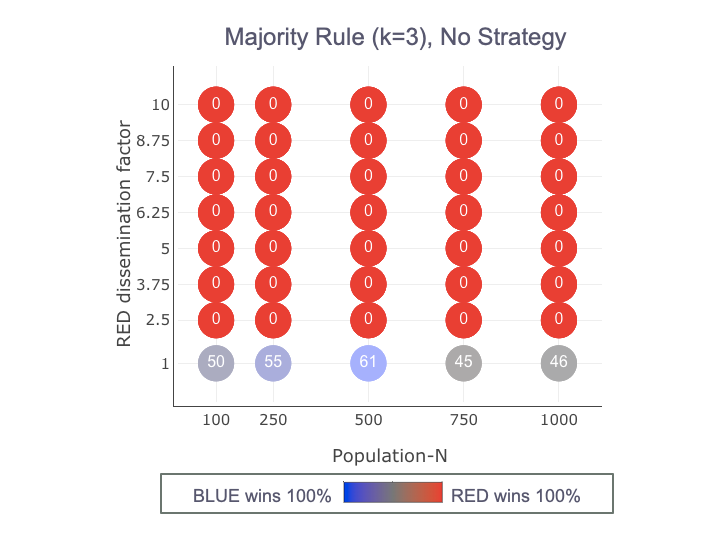
\includegraphics[trim={3cm 0 0 0},clip,scale=0.4]{images/Chart-Maj-k3-NoStrategy.png}
%       \caption{No-strategy, Majority rule (k=3). Similar to Voter model without strategy, in Majority Rule with symmetric quality we get no side that always win. We also did experiments using Majority rule with k=5 and k=7 without strategy and the results are similar to this chart.}
%       \label{fig:nostra-k3}
%   \end{figure}
   
%   \begin{figure}[thpb]
%       \centering
%       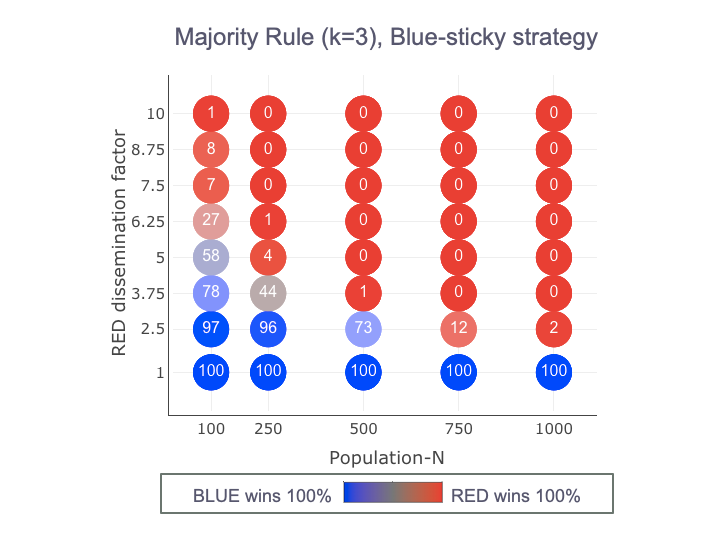
\includegraphics[trim={3cm 0 0 0},clip,scale=0.4]{images/Chart-Maj-k3-BlueSticky.png}
%       \caption{Blue-sticky defence strategy, Majority rule (k=3). Here the result is getting more interesting as Blue  was able to defeat Red who has up to 2.5 times of the quality (with Population-N = 100 and 200), and managed to prevent Red from winning despite Red quality is 5 times of Blue (with Population-N = 100). As the population grows, Blue's ability to win against Red is decreasing. }
%       \label{fig:sticky-k3}
%   \end{figure}

%   \begin{figure}[thpb]
%       \centering
      
%       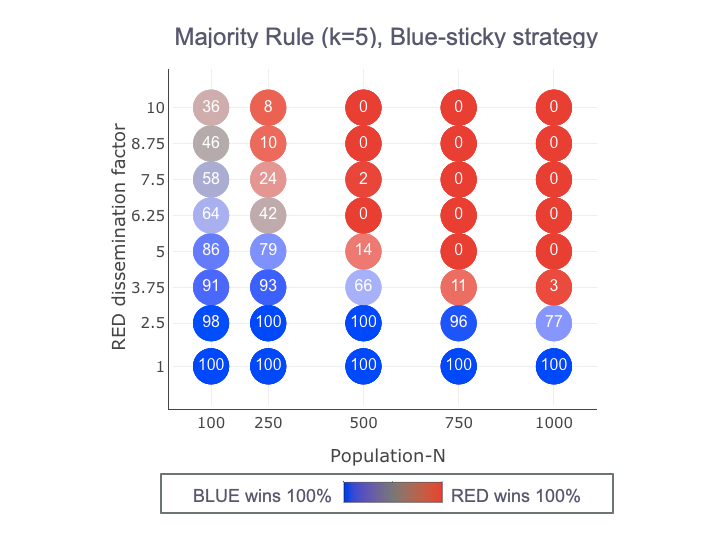
\includegraphics[trim={3cm 0 0 0},clip, scale=0.4]{images/Chart-Maj-k5-BlueSticky.png}
%       \caption{Blue-sticky defence strategy, Majority rule (k=5). The ability of Blue to win over Red extends to larger quality ratio as now we see in Population-N = 100 Blue always win at quality ratio of 5 and sometimes win at quality ratio of 7.5, while on Population N=1000 Blue always win
%       at quality ratio of 2.5 as compared to always lose in previous chart with k=3. }
%       \label{fig:sticky-k5}
%   \end{figure}

%   \begin{figure}[thpb]
%       \centering
%       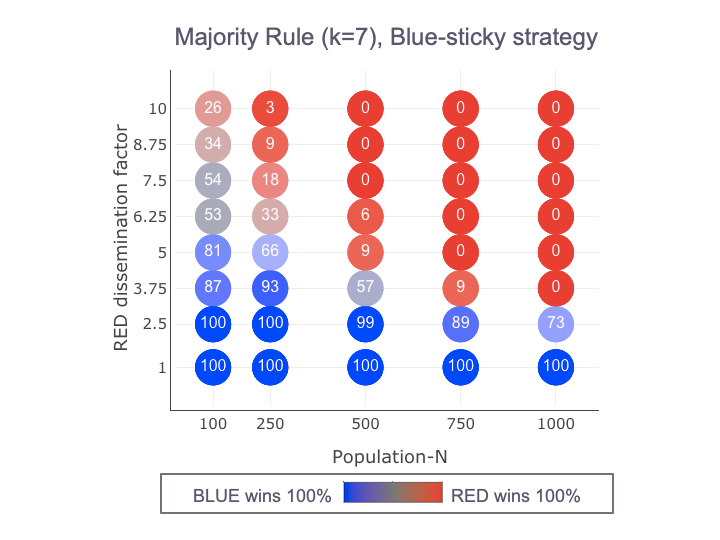
\includegraphics[trim={3cm 0 0 0},clip,scale=0.4]{images/Chart-Maj-k7-BlueSticky.png}
%       \caption{Blue-sticky defence strategy, Majority rule (k=7). The chart shows more convincing result where Blue managed to win against Red who has the quality ratio 10 times higher with Population-N = 100, while with Population-N=1000, although Red still wins at quality ratio of 5, the shade of the red circle is paler as compared to previously shown in k=3 chart.}
%       \label{fig:sticky-k7}
%   \end{figure}


\begin{figure*}
  \subfloat[]{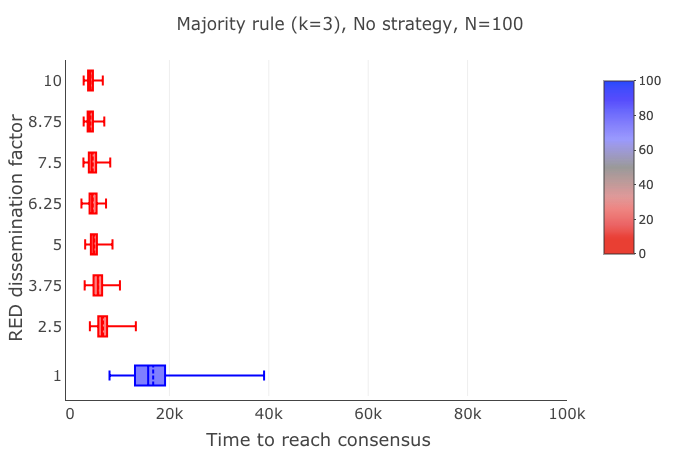
\includegraphics[width=0.46\textwidth]{images/NS-NCA-N100-k3.png} 
  \label{fig:no_str-k3}}
  \hfill
  \subfloat[]{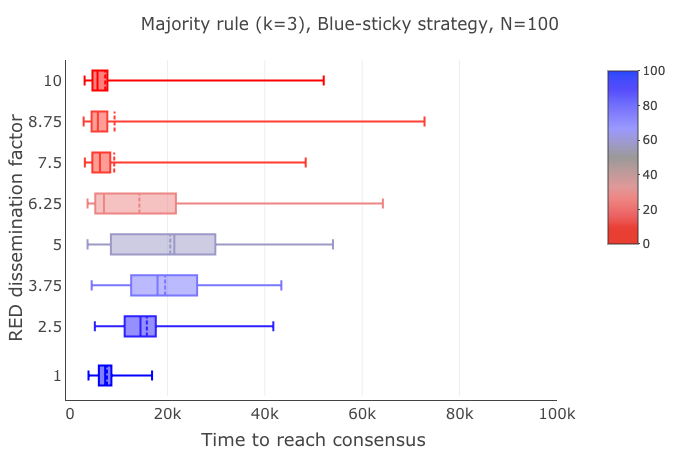
\includegraphics[width=0.46\textwidth]{images/BS-NCA-N100-k3.png} 
  \label{fig:sticky-N100k3}}
  %\\
  \caption{Boxplot plot of consensus time  with the majority model: (a)  no strategy and $k=3$, (b) blue strategy and $k=3$. This figure uses the same color-code convention used in Figure~\ref{fig:voter}.}
  \end{figure*}
  \begin{figure*}
  \subfloat[]{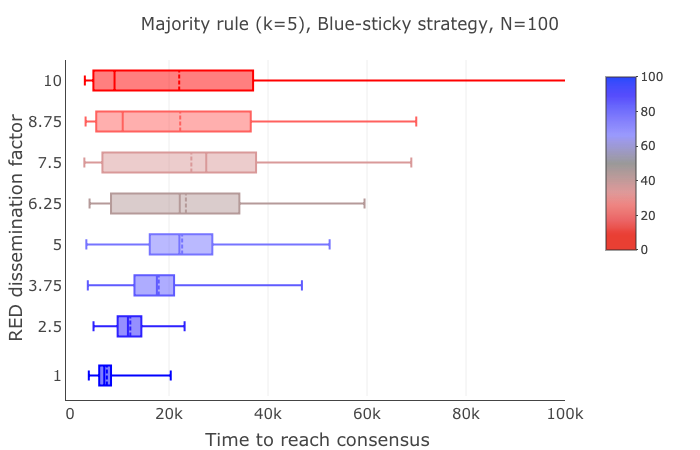
\includegraphics[width=0.49\textwidth]{images/BS-NCA-N100-k5.png} 
  \label{fig:sticky-N100k5}}
  \hfill
  \subfloat[]{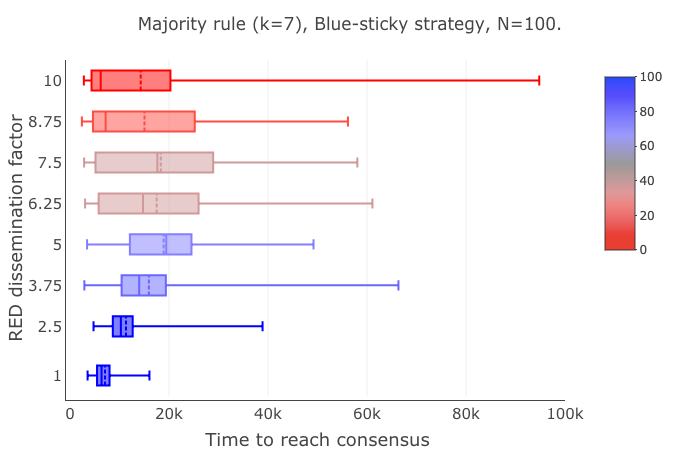
\includegraphics[width=0.49\textwidth]{images/BS-NCA-N100-k7.png} 
  \label{fig:sticky-N100k7}}
  \caption{Boxplot plot of consensus time  with the majority model: (a) blue strategy and $k=5$,(b) blue strategy and $k=7$. This figure uses the same color-code convention used in Figure~\ref{fig:voter}.}
  %\label{fig:majorityBoxplot100}
\end{figure*}

\begin{figure*}
  
  \subfloat[]{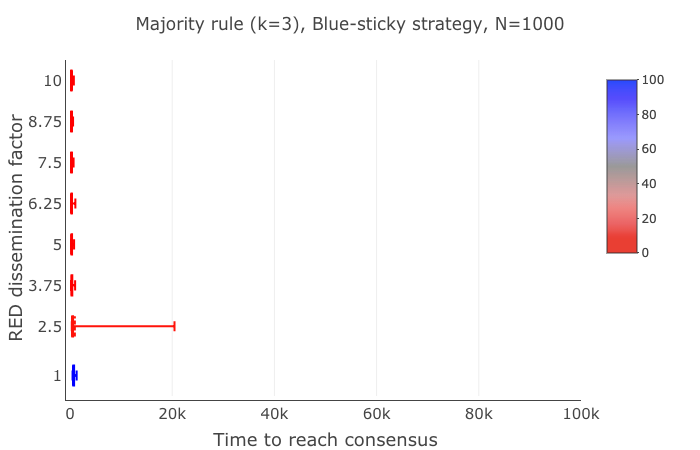
\includegraphics[width=0.49\textwidth]{images/BS-NCA-N1000-k3.png} 
  \label{fig:sticky-N1000k3}}
  \hfill
  \subfloat[]{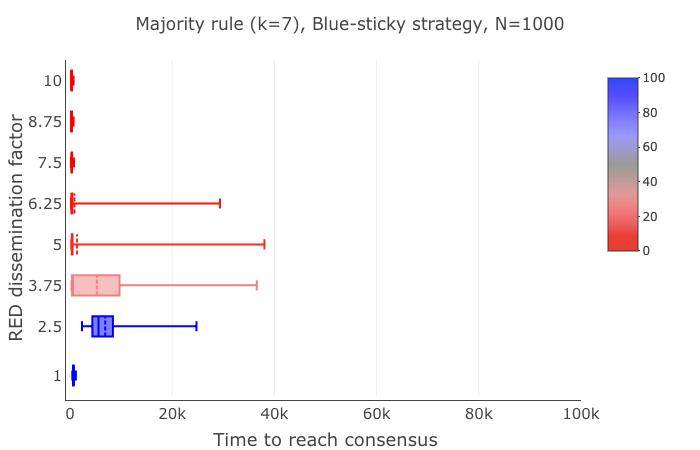
\includegraphics[width=0.49\textwidth]{images/BS-NCA-N1000-k7.png} 
  \label{fig:sticky-N1000k7}}
  \caption{Boxplot plot of consensus time  with the majority model: (a)   blue strategy and $k=3$ and (b) blue strategy and $k=7$. This figure uses the same color-code convention used in Figure~\ref{fig:voter}.}
  \label{fig:majorityBoxplot1000}
\end{figure*}

As expected, if no strategy is applied, the option with higher dissemination (RED) is winning for both the voter (Fig.\ref{fig:nostra-voter}) and the majority voting models (Fig.\ref{fig:nostra-k3}). If the two options RED and BLUE have the same dissemination (corresponding  to RED factor $1$) the consensus state is roughly $50\%$ of the times on RED  and $50\%$ of the times on  BLUE. This result, called "symmetry breaking" is well known from the literature. It discloses the tendency to converge to a bistable asymmetric  state (in our case consensus to either RED or BLUE), even if starting from a symmetric configuration (in our case, same dissemination factor for both RED and BLUE), due to stochastic fluctuations. The small divergence from $50\%$ observed in the majority rule case (Fig.\ref{fig:nostra-k3}) can be explained by stochasticity, due to the fact that the majority rule is less \emph{accurate} as a collective decision making mechanism~\cite{valentini|ferrante|hamann|dorigo:2015}.  

If, on the contrary, the sticking strategy is deployed, very different effects can be observed, depending on the voting model. If using the voter model, when the two options have the same dissemination factor, the BLUE option is always winning,  independently on the population size $N$ (Fig.\ref{fig:sticky-voter}). On the other hand,  if the RED dissemination factor is higher than the BLUE one, the RED option is always winning, despite the Blue-sticky strategy (Fig.\ref{fig:sticky-voter}). So in this case, the Blue-sticky strategy is effective only in the case the two options have the same dissemination factor, and starts to be ineffective as soon as the dissemination factor of RED option is larger than the BLUE one, at least for the range of considered parameters. 

More interestingly, if the majority voting model is implemented, the Blue-sticky strategy is revealing to be more  effective to drive the consensus to BLUE option, also  for relatively higher dissemination factor values of RED. The results for the three values of $k$  here investigated are reported in  Fig.\ref{fig:sticky-k3}, \ref{fig:sticky-k5}, \ref{fig:sticky-k7}. As evident from the figures, in the case with RED dissemination factor equal to $1$, the Blue-sticky strategy is effective to make the BLUE agents win, as in the voter model. But the Blue-sticky strategy is still effective also for RED dissemination factor $2.5$ and  population size $N=100$. This is true for all the considered $k$ values $[3, 5, 7]$. Focusing to $N=100$, when $k$ is increasing, the Blue-sticky strategy is effective even for increasingly higher dissemination factors: Comparing Fig.\ref{fig:sticky-k3}, \ref{fig:sticky-k5}, \ref{fig:sticky-k7}, we can observe that the indifference curve (that is the boundary where in 50\% of cases the consensus  is achieved to the BLUE option and in the remaining 50\% of cases to the RED option) is reached at RED dissemination factor $5, 7.5, >7.5$ for $k=3, 5, 7$ respectively. For larger population sizes $N$, the Blue-sticky strategy is less resilient to higher values of the RED dissemination factor, with this effect being less pronounced for higher values of $k$. We believe this is an effect of increased density, where RED agents can successfully infiltrate static Blue-sticky clusters when the density is high, and influence the local majority, an effect that can be attenuated by increasing $k$ which effectively increases the size of the local majority and makes it more robust to RED attacks. We plan to investigate better the effect of density and of $k$ in future work.

% We observe also that the cases $k=5$ (Fig.\ref{fig:sticky-k5}) and $k=7$ (Fig.\ref{fig:sticky-k7}) show similar results. This can be interpreted as an effect of ....


We also study how the time to reach consensus is affected by the various parameters.  In particular a boxplot representation of time has been used, varying the dissemination factor. The colors of boxplot follows the same conventions of heatmaps. This study has been done for different population sizes ($N=100, 250, 500, 750, 1000$) and voting models (voter, majority with $k=3,5,7$). The voter model is very accurate in reaching the consensus, mostly for large population sizes, as already known in literature. However, the consensus is reached only to the RED option, as already discussed; the consensus to BLUE option is only achieved for dissemination factor $1$ as described above. Therefore, here we only show the results for majority model \footnote{Voter results are available upon request} with $N=100, N=1000$.
For small populations, the majority model achieves consensus with shorter times, as also known in literature: majority mechanism is usually faster than voter model, but less accurate~\cite{valentini|ferrante|hamann|dorigo:2015}. In absence of blue sticky strategy the consensus to BLUE is achieved only with dissemination factor $1$ (Fig.\ref{fig:no_str-k3}). In majority model,  the number of voting neighbors of each agent, i.e. $k$, is a critical parameter in the decision making mechanism. This parameter plays a crucial role in small systems ($N=100$), particularly for very  large dissemination factors ($6$ and above), where the RED option wins: comparing Fig.\ref{fig:sticky-N100k3} ($k=3$), Fig.\ref{fig:sticky-N100k5} ($k=5$) and Fig.\ref{fig:sticky-N100k7} ($k=7$), the larger $k$, the larger is the variability of time necessary to reach the consensus. This can be easily explained because in small populations and high $k$ values, it is hard to find $k$ neighbors, due to the low density of agents, and agents that do not perceive at least $k$ neighbors do not change opinion. For lower dissemination factors (below $6$), where consensus to BLUE is achieved, there is no strong dependency on $k$ value. Here the blue-sticky strategy shows its effectiveness. The blue clusters trigger the consensus and favor the availability of $k$ neighbors, speeding up the majority mechanism. 

The other important factor is  the population size $N$, being the consensus times much longer for small systems ($N=100$), compared with larger systems ($N=500, 1000$), as evident comparing Fig.\ref{fig:sticky-N100k3} ($N=100$, $k=3$) with Fig.\ref{fig:sticky-N1000k3}  ($N=1000$, $k=3$) and Fig.\ref{fig:sticky-N100k7} ($N=100$, $k=7$)  with Fig.\ref{fig:sticky-N1000k7}  ($N=1000$, $k=7$) . 
For larger population sizes the availability of $k$ neighbors is guaranteed by higher density values. Therefore, the majority model is much faster than in the case of small populations. 
%Introducing the collision avoidance has beneficial effects, decreasing the variability of consensus time. In cases where the consensus can be either to RED or to BLUE, the time scales of consensus are .... 

\subsection{Real Robot Experiment}
In the real robot runs, the swarm opinion converged completely to Blue on average in 13 minutes and 57 seconds. This test provided evidence of what was observed in the numerical simulations: when the dissemination of RED is higher than the one of BLUE, the BLUE robots can still achieve the consensus using the Blue-sticky strategy. A demonstration video showing one of the runs is available upon request (for anonymity during paper review).

%\url{https://www.youtube.com/watch?v=qei4u5GFKn8}.

   \begin{figure}[t]
      \centering
      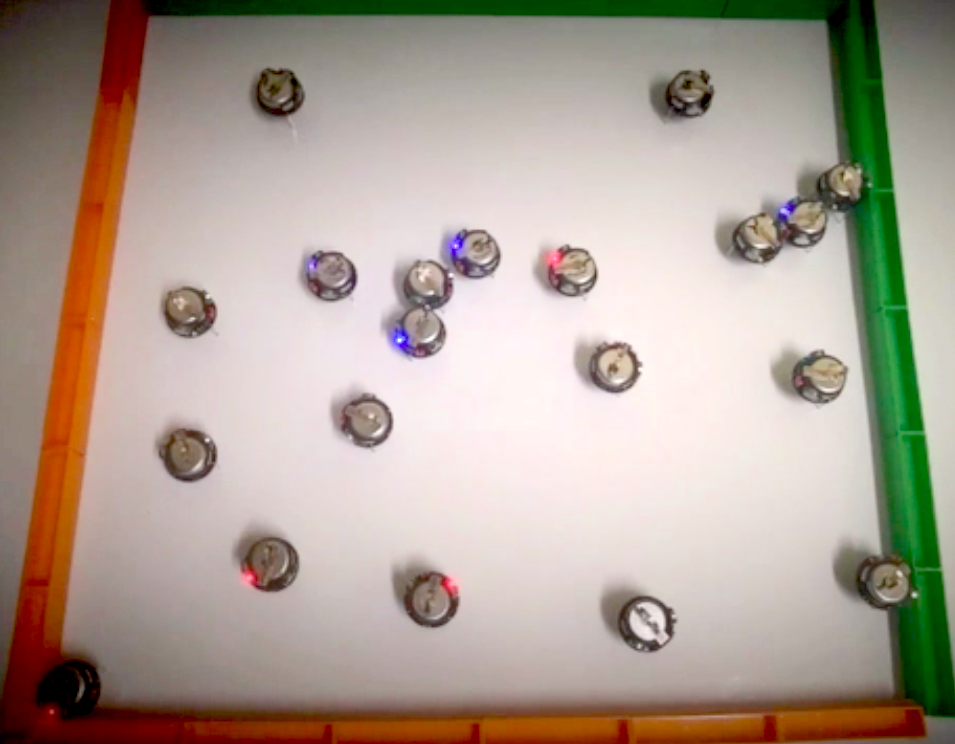
\includegraphics[scale=0.17]{images/Photo-Kilobots-Experiment.png}
      \caption{Experiment with 20 Kilobots on 50 cm by 50 cm arena}
      \label{fig:kilobots}
   \end{figure}
   
\section{CONCLUSIONS}
\label{sec:conclusions}

In this paper, we study a mechanism to increase the resiliency of a swarm of agents performing collective decision making, subject to attacks represented by the malicious exploitation of the positive feedback modulation. Two options, BLUE and RED, are assumed to have two different dissemination factors, that is two different times of dissemination of their opinions. The BLUE option is characterized by a dissemination factor that is lower than the RED option. Nevertheless, the BLUE option wants to defend its opinion, against the attacks of the RED option. The BLUE option can still win the consensus, when the agents with such opinion use a  spatial strategy through which they stay in place and stick the attacker, once it is converted from RED to BLUE. %stay in place. 
This mechanism is  inspired by the defence strategy used by stingless bees, that use some special resin to stick attackers in order to defend themselves. %Similarly,  here a group of robots is able to defend itself against attacker robots. 
To simulate this behaviour, we divided a swarm in two initially equally populated sets: RED and BLUE. The RED randomly move inside the experimental arena, while the BLUE stick in their original position. In the collective decision making mechanism, a defender (BLUE) is able to convert the attacker (RED) to change its opinion, sticking it in its last position. In this way the attacker (RED) becomes a defender (BLUE). Through this mechanism, an overall agreement to the defender (BLUE) or attacker (RED) option is always reached. From a design perspective, the final aim is to identify the parameters to obtain  the agreement to the defender's opinion. Comparing two different decision making mechanisms, voter and majority models, we found that  only the majority rule allows to get consensus with very high probability even when RED is able to disseminate for longer amount of times, but that the voter is able to break the symmetry towards the BLUE option only when the two options are disseminated for an equal amount of time.  %This happens even when the dissemination factor of attackers is much larger than the dissemination factor of attackers. 
The majority decision making rule together with the blue-sticky strategy is resilient to attackers having a dissemination factor up to $5$ times the dissemination factor of defenders. Moreover, this strategy is effective also in terms of time to reach the consensus: the forming clusters speed up the consensus achievement to BLUE option. 

We can conclude that, if agents are attacked by more aggressive agents (with higher dissemination factor), a good strategy for them to win is to stop where they are and progressively form clusters. This study can be particularly relevant for patrolling and surveillance applications. The fact that small systems are more resilient to external attacks, compared with larger systems make this strategy suitable to be applied in real surveillance swarms of agents.

In the next studies, we will investigate the spatial distribution of agents, where agglomeration of blue agents is expected.  Finally, we note that the Blue-sticky can be considered a rudimentary aggregation behaviour, as it produces clusters, thus it is in our agenda to study the coupling of collective decision making with other collective behaviours that produce different spatial correlations, such as collective motion or pattern formation. 

%\addtolength{\textheight}{-12cm}   % This command serves to balance the column lengths

%%%%%%%%%%%%%%%%%%%%%%%%%%%%%%%%%%%%%%%%%%%%%%%%%%%%%%%%%%%%%%%%%%%%%%%%%%%%%%%%
% \section*{APPENDIX}

% Appendixes should appear before the acknowledgment.

\section*{ACKNOWLEDGMENT}

We acknowledge Middlesex University Dubai for the lab facilities provided for Kilobots experiments.

%%%%%%%%%%%%%%%%%%%%%%%%%%%%%%%%%%%%%%%%%%%%%%%%%%%%%%%%%%%%%%%%%%%%%%%%%%%%%%%%
\bibliographystyle{plain}
\bibliography{cdm}
\end{document}



